\documentclass[12pt,twoside]{article}
\usepackage{jmlda}
\usepackage{graphics}
%\NOREVIEWERNOTES
\title
    %[Образец оформления статьи для публикации] % Краткое название; не нужно, если полное название влезает в~колонтитул
    {Мультимоделирование как универсальный способ описания выборки общего вида}
\author
    %  [Логинов~Р.\,А.] % список авторов для колонтитула; не нужен, если основной список влезает в колонтитул
    {Логинов~Р.\,А., Адуенко~А.\,А., Стрижов~В.\,В.} % основной список авторов, выводимый в оглавление
    % [Логинов~Р.\,А., Адуенко~А.\,А., Стрижов~В.\,В.] % список авторов, выводимый в заголовок; не нужен, если он не отличается от основного
\thanks
    {Работа выполнена при финансовой поддержке РФФИ, проект \No\,00-00-00000.
   Научный руководитель:  Стрижов~В.\,В.
   Задачу поставил:  Стрижов~В.\,В.
    Консультант:  Адуенко~А.\,А.}
\email
    {logipamar@yandex.ru}
%\organization
%    {$^1$Организация; $^2$Организация}
\abstract
    {В случае неоднородных данных в машинном обучении использования одной модели недостаточно. Для выявления этого используют комбинации нескольких моделей - мультимодели. Работа нацелена на то, чтобы изучить по последовательности постепенно приходящих данных эволюцию представлений о модели. Рассмотреть, в какие моменты предпочтительнее разветвлять одну модель, а также какими критериями пользоваться для объединения ещё недообученного ответвления с имеющимися моделями. Исследования проводятся на синтетических данных из многоуровневой модели или смеси распределений.

\bigskip
\textbf{Ключевые слова}: \emph {мультимоделирование, бинарная классификация, эволюция моделей, адаптивное обучение}.}
\titleEng
    {JMLDA paper example: file jmlda-example.tex}
\authorEng
    {Author~F.\,S.$^1$, CoAuthor~F.\,S.$^2$, Name~F.\,S.$^2$}
\organizationEng
    {$^1$Organization; $^2$Organization}
\abstractEng
    {This document is an example of paper prepared with \LaTeXe\
    typesetting system and style file \texttt{jmlda.sty}.

    \bigskip
    \textbf{Keywords}: \emph{keyword, keyword, more keywords}.}
\begin{document}
\maketitle
%\linenumbers

\section{Введение}

Работа посвящена исследованию решения задач бинарной классификации при помощи мультимоделей. Решение этой задачи может быть использовано в вопросах кредитного скоринга [], медицинской диагностики [], предсказания качества продукции и других областях. В некоторых задачах встречаются данные, для описания которых требуется вводить несколько моделей. Например, для задачи кредитного скоринга важность признаков в модели может отличаться в зависимости от региона заявителя. Как пример, многодетность может быть положительным параметром для более благополучных регионов и отрицательным для менее состоятельных. Тогда используют решающее правило о разделении выборки на кластеры, а затем на каждом из них строят отдельную модель. Такой подход называют многоуровневой моделью.

Один из алгоритмов построения и обучения оптимальной модели, основанный на байесовском выводе и ЕМ-алгоритме, описан в [Aduenko-main]. Более того, известна процедура выявления максимального числа необходимых моделей, а также построена функция, которая, в отличие от методов, основанных на дивергенциях Брегмана и KL-дивергенциях, позволяет оценить различимость двух моделей.

Однако этот алгоритм рассматривает выборку как статическую и известную заранее. В прикладных задачах появляются данные, имеющие временную структуру. Из-за этого на одном и том же объекте ответ с течением времени может различаться. Таким образом целью работы является исследование эволюции модели во времени. Более того, в статье приведены эксперименты, выявляющие необходимый размер выборки, которую возможно отделить для построения новой модели. Подобные результаты планируется получить на синтетических данных, где временная структура будет различной: случайный выбор модели и непрерывные отрезки во времени, на которых поступает каждая модель.

В упомянутой работе такая оптимизация алгоритма не приведена, и новый подход позволяет улучшить качество мультимоделей в задачах бинарной классификации.  

Предлагается построить модификацию этого алгоритма, взяв его за основу. Один из методов заключается в том, чтобы для новой модели учитывать лишь ту часть выборки, которая поступила последней. Размер этой части является гиперпараметром и будет подобран на синтетических данных.

Затем полученный алгоритм предлагается сравнить с уже имеющимся как на построенных синтетических данных, так и на собранных в репозитории UCI данных о кредитном скоринге, бинаризованных данных о стоимости квартир и о качестве вина [].

\section{Постановка задачи}

Как уже отмечено, в работе рассматривается задача бинарной классификации. Это означает что изначально имеется некоторая выборка объектов. Объект представляется в виде пары $(\mathbf{x}, y)$, где $\mathbf{x} \in \mathbb{X} \subset \mathbb{R}^n$ - признаковое описание объекта, а $y \in \{0, 1\}$ - корректный класс объекта.

Соответственно, выборка обозначается $\mathfrak{D} = \{(\mathbf{x}_i, y_i)\}, i \in \mathcal{I} = \{1, ..., m\}$, а матрицей $\mathbf{X}$ обозначим матрицу объектов, у которой в строке с индексом $i$ будет содержаться признаковое описание объекта $\mathbf{x}_i$.

\begin{Def}
	\emph{Моделью бинарной классификации} будем называть параметрическое семейство функций $f$, отображающих декартово произведение множества значений признакового описания объектов $\mathbb{X}$ и множества параметров $\mathbb{W}$ в множество значений целевой переменной $\mathbb{Y} = \{0, 1\}$
\end{Def}

\begin{Def}
	\emph{Бинарным классификатором} называется отображение $f$ из множества признакового описания объектов $\mathbb{X}$ в пространство целевой переменной $\mathbb{Y}$
\end{Def}

\begin{Def}
	\emph{Вероятностным классификатором} называется условное распределение вида
	$$ q(y|\mathbf{x})\ :\ \mathbb{Y} \times \mathbb{X} \rightarrow \mathbb{R}^{+}$$
\end{Def}

Имея вероятностный классификатор, можно построить бинарный классификатор по следующему принципу:

$$f(\mathbf{x}) = I\{q(1|\mathbf{x}) > T\},$$

где $T \in (0, 1)$ - \emph{порог классификации}, который является одним из гиперпараметров модели.

Для оценки качества модели в общем случае необходима функция ошибки, не зависящая от порога классификации. Для этого подходит AUC ROC - площадь под ROC-кривой, описание которой имеется в []

Чтобы избежать проблемы переобучения, множество объектов представляется в виде объединения обучающей и тестовой выборки: $\mathfrak{D} = \mathfrak{D}_{test} \sqcup \mathfrak{D}_{train}$.

Соответственно определяются и множества индексов:

$$ \mathfrak{D}_{train} = \{(\mathbf{x}_i, y_i)\}, i \in \mathcal{I}_{train} \subset \mathcal{I} $$
$$ \mathfrak{D}_{test} = \{(\mathbf{x}_i, y_i)\}, i \in \mathcal{I}_{test} \subset \mathcal{I} $$

Если же объекты отсортированы во времени, то обучающая выборка должна идти во времени раньше, поэтому рассматриваются следующие множества в качестве индексных:

$$ \mathcal{I}_{train} = \{1, ..., t\} $$
$$ \mathcal{I}_{test} = \{t + 1, ..., m\} $$

Как было отмечено, данные могут не описываться одной моделью. Поэтому для решения задачи классификации рассмотрим множество $\mathbb{M} = \{f_i\}, i \in \mathfrak{M}$ - множество используемых моделей, где каждый из $f_i$ - вероятностный бинарный классификатор.

\begin{Def}
	Выборкой \emph{с временной структурой} называется такое множество объектов $\mathfrak{D} = \{\mathbf{x}_i, y_i)\}, i \in \mathcal{I}$, на котором задано отображение $t: \mathbb{X} \rightarrow \mathbb{N}$, определяющее время прибытия объекта, такое, что
	$$ \forall i, j \in \mathcal{I}:\ i < j\ \Rightarrow t(\mathbf{x}_i) < t(\mathbf{x}_j) $$
\end{Def}

Целью обучения является задать множество моделей $\mathbb{M}$, множество параметров $\mathbf{w}$ для каждой из них, причём каждый из параметров должен быть функцией от времени прибытия объекта, поскольку рассматривается эволюция модели. Обозначим эти параметры как функции  $\{\mathbf{w}_i(t)\}, i \in \mathfrak{M}$

Более того, требуется определить, по какой из моделей считать ответ на объекте. Для этого необходимо построить отображение $\mathcal{M}: \mathbb{X} \rightarrow \mathfrak{M}$ из множества признакового описания объектов в множество индексов моделей, которое задаст выбранную модель.

Задав такие множества, становится возможным построить классификатор $f_{mult}$ следующим образом:

\begin{enumerate}
	\item Выбрать модель при помощи отображения $\mathcal{M}$
	\item Вычислить значения параметров, учитывая время прихода объекта $t(\mathbf{x})$
	\item Получить предсказание обученной выбранной модели
\end{enumerate}

$$ f_{mult}(\mathbf{x}) = f_{\mathcal{M}(\mathbf{x})}(\mathbf{w}_{\mathcal{M}(\mathbf{x})}(t(\mathbf{x})), \mathbf{x}) $$

Таким образом, требуется решить следующую оптимизационную задачу, решение которой будем называть \emph{обучением мультимодели}:

\begin{align*}
\arg\max&\ AUC\-ROC(\mathfrak{D}_{train}, f_{mult}(\mathcal{M}, \mathbf{w})) \\
    s.t.&\ \mathcal{M}: \mathbb{X} \rightarrow \mathfrak{M} \\
        &\ \mathbf{w} = \mathbf{w}(t) = \{\mathbf{w}_i(t)\}_{i \in \mathfrak{m}}
\end{align*}

\textbf{Описание отдельных моделей}. В качестве моделей для множества $\mathbb{M}$ будут рассматриваться модели логистической регрессии с вектором весов $\mathbf{w} \in \mathbb{R}^n$ и набором гиперпараметров $\mathbf{\mu}$:

$$ p(y, \mathbf{w} | \mathbf{x}, \mathbf{\mu}) = \sigma(y\mathbf{w}^\top \mathbf{x})p(\mathbf{w} | \mathbf{\mu}) $$

Здесь $\sigma(x) = \frac{1}{1 + e^{-x}}$.

Каждая из моделей будет обучаться методом максимальной обоснованности, который описан в [1]

\bigskip
\textbf{Природа данных}. Исследование будет проведено на синтетических данных для того, чтобы построенная модель соответствовала получаемым данным. Будут рассмотрены 2 случая, при которых становится целесообразным использование мультимоделей.

Первый случай - это случай \emph{многоуровневой модели}. В данном случае при генерации будет использован набор правил, который определит, к какой группе объектов (к какому кластеру), будет принадлежать объект $\mathbf{x}$. После этого для каждого кластера буден задан свой вектор весов, по которому будет вычисляться вероятность принадлежности конкретному классу. Затем, если эта вероятность выше некоторого порога, объекту будет сопоставлен класс $1$, иначе - $-1$.

Другой случай - случай \emph{смеси моделей}. Пусть данные генерируются из $k$ моделей, для каждой из которых задан вектор весов. Пусть также есть вектор $\mathbf{\pi} \in \mathbb{R}^k$, где $\mathbf{\pi}_i$ задаёт вероятность генерации объекта из модели с индексом $i$. Этот вектор будет сгенерирован из симметричного распределения Дирихле.

В каждом из случаев вектора весов будут генерироваться из нормального распределения с нулевым средним и диагональной матрицей ковариаций. Именно такие распределения будут рассматриваться в качестве априорных при обучении классификаторов в данной работе. 

\section{Базовый эксперимент}

В качестве базового алгоритма использовался алгоритм для построения мультимоделей, описанный в [1]. Для самого простого случая рассматривается многоуровневая модель с двумя группами рассматриваемых объектов. В данном эксперименте для удобства визуализации рассматривается $\mathbb{X} = \mathbb{R}^2$. 

В задачах, в которых используются многоуровневые модели, правила, по которым объекты разделяются по группам, зафиксированы заранее. Поэтому изначально обучающая выборка разделена на кластеры:

$$ \mathfrak{D} = \mathfrak{D}_1 \sqcup \mathfrak{D}_2 \sqcup ... \sqcup \mathfrak{D}_K $$

Поэтому для обучения многоуровневой модели требуется лишь обучить логистическую регрессию на каждой выборке $\mathfrak{D}_i$, чтобы затем получить оптимальные веса $\mathbf{w}_i$ для каждой из моделей. Чтобы получить ответ на тесте, достаточно вычислить правило, по которому объект относится к кластеру, а затем получить предсказания, используя фиксированную для данного кластера модель.

Для базового эксперимента выбран параметр  $K = 2$. Цель - рассмотреть, насколько будут отличаться предсказания при использовании многоуровневой модели и одиночной логистической регрессии. Также оценить уровень значимости для гипотезы различимости одиночной и многоуровневой модели при помощи алгоритма \emph{s-score}, описанного в [1].

\begin{figure}
        \center{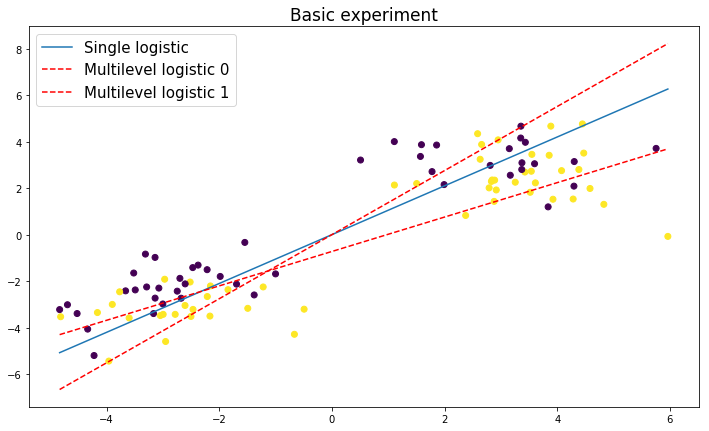
\includegraphics[width = 0.8\textwidth]
        {PresBasic.eps}}
        \caption{\label{fig:my-label} Сравнение одиночной и многоуровневой модели}
\end{figure}

Видим, что использование мультимодели в этом конкретном случае даёт улучшение в точности классификации. Две прямые в данном случае хорошо разделяют точки разных цветов, соответсвтующие различным классам. Однако результат \emph{s-score} оказывается статистически незначимым. Возможно, такой эффект объясняется недостаточным размером выборки для отвержения гипотезы неразличимости моделей. Поэтому одной из дальнейших целей исследования является выявление размера выборки, при котором можно выделить в данных новую модель.

Однако в случае, при котором закономерности в данных меняются с течением времени, объекты, имеющие одинаковые признаковые описания, но разные ответы на них, вносят шум в построенную модель, и для улучшения качества классификации требуется не учитывать в модели подобные предыдущие случаи. Более того, если данный приходят последовательно, для нового прогноза возможно использовать только те данные, которые были получены до поступления нового объекта.

Таким образом, дальнейший эксперимент должен включать в себя рассмотрение новой синтетической выборки с меняющейся разделяющей прямой, а также оценку качества с использованием базовой модели, обученной на соответствующем префиксе.

\section {Описание модификации алгоритма}

В работах, учитывающих изменение модели во времени, применяют либо анализ временных рядов [], который зачастую рассматривается для задач одномерной регрессии и учитывает наличие множества других признаков лишь в специфичных случаях, либо анализ последовательностей []. Задача анализа последовательности формализуется следующим образом: пусть аналогично поставленной выше задаче зафиксирована обучающая выборка $\{(\mathbf{x}_i, \mathbf{y}_i)\}_{i = 1}^N$. Отличие заключается в том, что каждый из $\mathbf{x}_i \in \mathbb{X}^k$ - это последовательность признаковых описаний объектов, а для задачи классификации $\mathbf{y}_i \in \{1, -1\}^k$ - ответы на этой последовательности.

Обученная модель может учитывать предыдущие объекты и предсказанные ответы на них, что и требуется для учёта временной структуры. Одним из распространенных методов является метод скользящего окна. Для зафикисированного гиперпараметра - половины длины окна $d$, для каждого объекта $\mathbf{x}_{i,j} \in \mathbb{X}$ рассматривается стандартная задача обучения с учителем. Но в качестве дополнительных признаков рассматриваются также описания ближайших расположенных объектов внутри обучающей выборки, а именно $\mathbf{x}_{i, j - d}, ..., \mathbf{x}_{i, j + d}$.

Существует также модифицированная версия этого алгоритма, в которой в пространство признаков также вводятся предсказания модели на $d$ предыдущих объектах ($\mathbf{y}_{i, j - d}, ... \mathbf{y}_{i, j - 1}$).

Однако все эти методы более, чем в $d$ раз увеличивают размерность пространства признаков. При этом учитываются только близкие во времени объекты. Для рассматриваемой задачи же требуется метод, который будет как убирать из рассмотрения моделью нерелевантные данные, так и дообучать модель при помощи новых объектов.

Идею скользящего окна можно адаптировать для построения нового метода, который позволит учесть заявленные требования к модели. Пусть $D$ - гиперпараметр, размер окна (именно всего окна, а не его половины). Он подбирается на основании экспериментов с базовым алгоритмом. Длина окна должна быть такой, чтобы модель, обученная лишь на данных внутри окна, могла стать статистически значимо отличимой от текущей модели.

Пусть $\mathfrak{D}$ - выборка, заданная в постановке задачи. Разобьём отсортированные по времени данные на группы подряд идущих объектов по $D$ штук. Таким образом, в группу $G_i$ попадут объекты $\{\mathbf{x}_{j}:\ j \in [Di, D(i + 1) - 1]\}$. Под мультимоделью в дальнейшем понимается один из двух случаев - многоуровневая модель или же смесь моделей.

Предполагается, что существует обучаемая мультимодель $f$ с параметрами $\mathbf{w}$, которая обучена на данных, пришедших до текущего момента времени. Данные рассматриваются по группам. Пусть в данный момент рассматривается группа $G_i$. Предлагается сделать для этой группы следующие действия:

\begin{enumerate}
\item Построить мультимодель $f_0$, обучив её на данных из $G_i$;
\item Вычислить \emph{s-score} для оценки различимости $f$ и $f_0$;
\item Если различимость не отвергается, то дообучить $f$ на данных из $G_i$;
\item Если отвергается, заменить $f$ на $f_0$.
\end{enumerate}

Подразумевается, что если накопились данные, которые описываются значимо отличимой мультимоделью, рассматривать предыдущие данные уже не имеет смысла, ведь модель могла стать обученной на неверных для текущего момента времени ответах.

\section {Вычислительных эксперимент и анализ ошибки}

\subsection {Генерация синтетической выборки}

Как и написано выше, эксперимент проводится для случая многоуровневой модели. А это значит, что для начала необходимо задания правила, по которому объекты будут отнесены к тому или иному кластеру. Для удобства визуализации выбран двумерный случай. Пусть точками из первого кластера считаются те, которые находятся в первой четверти плоскости координат, а точками из второго - точки из третьей четверти. Допустим также, чтобы данные внутри одного кластера генерировались из многомерного нормального распределения с заданными заранее параметрами. Тогда при выборе центров кластеров, достаточно отдаленных от нуля координат, вероятность того, что точки, сгенерированные по одному правилу, попадут в противоположный кластер, становится мала.

Вторым шагом для построения выборки является  задание разделяющих прямых в каждом из случаев. И при этом должно наблюдаться изменение разделяющего правила по времени. В этом примере изменение задаётся при помоши поворота по часовой стрелке разделяющей прямой вокруг центра кластера. Изначально прямые расположены перпендикулярно друг другу для того, чтобы было оправданным использование мультимоделирования, - в данных есть неоднородность.

В такой модели построения есть два основных параметра. $\alpha$ - угол, на который на каждом этапе поворачиваются прямые, $C$ - количество элементов, которые добавляются в каждый кластер после поворота. 

\subsection {Подбор размера выборки}

Согласно конструкции алгоритма, чтобы изменение закономерности в данных было зафиксировано, необходимо отвержение гипотезы о неразличимости модели, построенной на новых данных, и текущей имеющейся модели. Поэтому необходим размер новой выборки, достаточный для отвержения. Однако этот размер выборки зависит от того, насколько различаются модели на двух этапах. Пусть задан угол поворота прямой  $\alpha$. Тогда при помощи семплирования можно вычислить можность критерия для гипотезы неразличимости, основанного на s-score. Зададим для эксперимента $\alpha = \frac{\pi}{12}$.

\begin{figure}
        \center{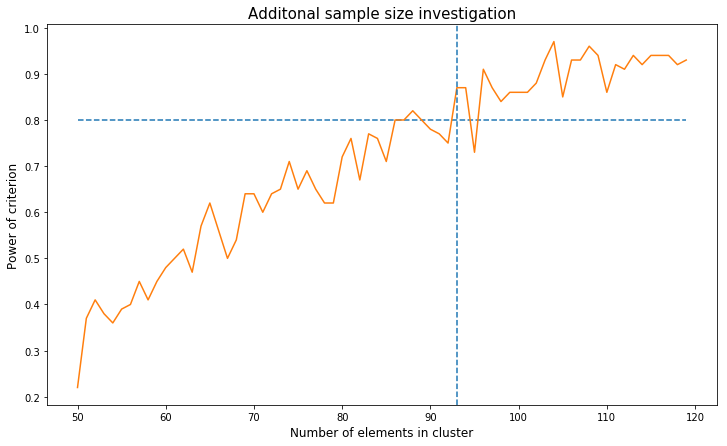
\includegraphics[width = 0.8\textwidth]
        {../report/PresPower.eps}}
        \caption{\label{fig:my-label} Мощность критерия неразличимости}
\end{figure}

Итоговый график оценок мощности изображен на рисунке 2. Зафиксируем параметр $C$ таким, чтобы мощность превосходила $0.8$. Например, подходит $C = 93$. Однако в этом случае, если задать для алгоритма размер окна $D = 93$, то на каждом шаге будет строиться новая модель, и предсказания с актуальным представлением о модели не смогут быть построены ни на одном шаге. Поэтому возьмём $D = 94$, а $C$ увеличим вдвое.

Будем генерировать данные до тех пор, пока прямые не пройдут весь круг. На рисунках 3-5 представлены новые данные на первом шаге и в середине генерации, а также все данные, наложенные друг на друга. Таким образом, зависимость закономерности от времени здесь очевидна, и предложенный алгоритм должен превосходить по качеству исходный.

\begin{figure}
        \center{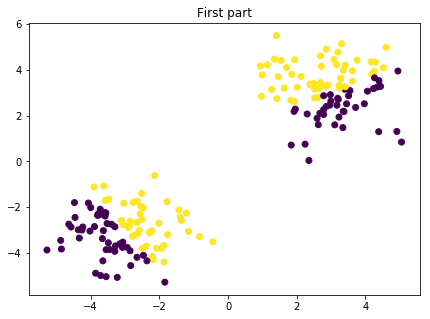
\includegraphics[width = 0.8\textwidth]
        {../report/PresData1.eps}}
        \caption{\label{fig:my-label} Первая часть датасета}
\end{figure}

\begin{figure}
        \center{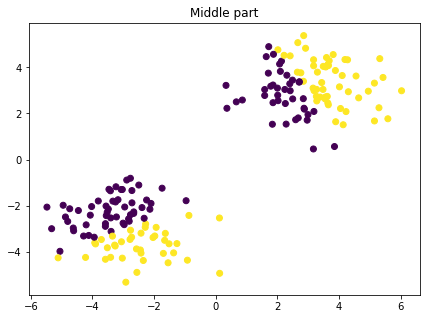
\includegraphics[width = 0.8\textwidth]
        {../report/PresData2.eps}}
        \caption{\label{fig:my-label} Блок данных из середины генерации}
\end{figure}

\begin{figure}
        \center{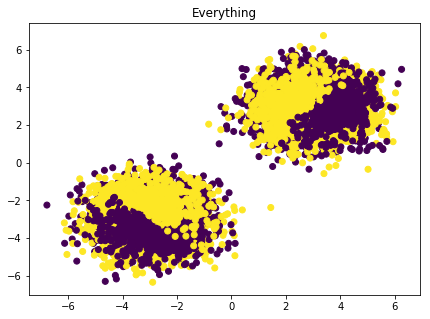
\includegraphics[width = 0.8\textwidth]
        {../report/PresDataAll.eps}}
        \caption{\label{fig:my-label} Итоговая выборка}
\end{figure}


\subsection {Результаты}

В эксперименте был использован заранее известный оптимальный параметр модели $D$. При этом при необходимости дообучения имеющейся модели, производилось обучение заново также и на имеющихся ранее данных. Полученные результаты, а именно  ROC-кривые, изображены на рисунках 6-7.

\begin{figure}
        \center{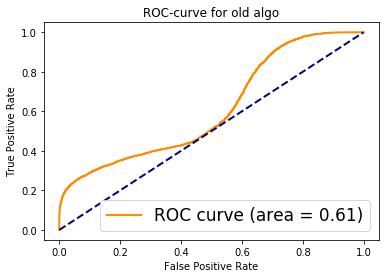
\includegraphics[width = 0.8\textwidth]
        {../report/PresRocOld.eps}}
        \caption{\label{fig:my-label} ROC-кривая для исходного алгоритма}
\end{figure}

\begin{figure}
        \center{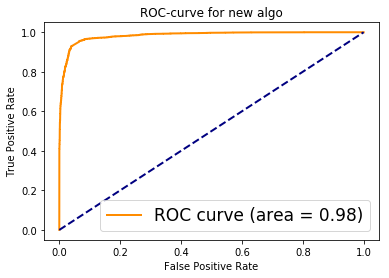
\includegraphics[width = 0.8\textwidth]
        {../report/PresRocNew.eps}}
        \caption{\label{fig:my-label} ROC-кривая для модифицированного алгоритма}
\end{figure}

Видим, что качество нового алгоритма заметно лучше. При этом наблюдается эффект, при котором ROC-кривая для базовой модели приближается к диагонали. Такой эффект может быть связан с тем, что в момент, когда разделяющие прямые повернулись на 180 градусов, предсказания на объектах с теми же признаками, что и у исходных, поменялись на противоположные.

\section {Заключение}

Таким образом, была рассмотрена задача мультимоделирования в случае изменения закономерности во времени. С учетом этой особенности данных был доработан исходный алгоритм, предложенный в базовой работе, в основе которого лежит проверка гипотезы неразличимости при помощи s-score. Была продемонстрирована эффективность данного алгоритма на синтетических данных.

Однако улучшение было получено лишь тогда, когда был известен оптимальный параметр. В общем случае при неверно подобранном размере окна есть риск ухудшения качества предсказания по сравнению с исходным алгоритмом.

Более того, ещё один недостаток заключается в том, что при перестроении модели часть данных перестает учитываться. И если в сгенерированном примере это было полезно, то на реальных данных даже устаревшие объекты помогают предсказывать целевую переменную. Один из вариантов учесть все имеющиеся данные - применение байесовского вывода, например, над функцией среднего и ковариационной функцией гауссовского процесса.

\bibliographystyle{unsrt}
\bibliography{jmlda-bib}
\begin{thebibliography}{1}

\bibitem{aduenko_main}
    \BibAuthor{Адуенко А.А.}
    \BibTitle{Выбор мультимоделей в задачах классификации}

\bibitem{window}
    \BibAuthor{Thomas G. Dietterich}
    \BibTitle{Machine Learning for Sequential Data: A Review}

\bibitem{adaptive}
    \BibAuthor{Craig Wilson et. al}
    \BibTitle{Adaptive Sequential Learning}

\bibitem{china}
    \BibAuthor{Ge Y., Jiang W.}
    \BibTitle{On consistency of Bayesian inference with mixtures of logistic  regression}

\bibitem{bishop}
    \BibAuthor{Christofer M. Bishop}
    Pattern recognition and machine learning.


\end{thebibliography}
% Решение Программного Комитета:
%\ACCEPTNOTE
%\AMENDNOTE
%\REJECTNOTE
\end{document}
